\documentclass[a4paper, 11pt]{article}
\usepackage{comment} % enables the use of multi-line comments (\ifx \fi) 
\usepackage{fullpage} % changes the margin
\usepackage[a4paper, total={7in, 10in}]{geometry}
\usepackage{amsmath,mathtools,mathdots}
\usepackage{amssymb,amsthm}  % assumes amsmath package installed
\usepackage{float}
\usepackage{xcolor}
\usepackage{mdframed}
\usepackage[shortlabels]{enumitem}
\usepackage{indentfirst}
\usepackage{hyperref}
\hypersetup{
	colorlinks=true,
	linkcolor=doc!80,
	citecolor=myr,
	filecolor=myr,      
	urlcolor=doc!80,
	pdftitle={Assignment}, %%%%%%%%%%%%%%%%   WRITE ASSIGNMENT PDF NAME  %%%%%%%%%%%%%%%%%%%%
}
\usepackage[most,many,breakable]{tcolorbox}
\usepackage{tikz}
\usepackage{caption}
\usepackage{kpfonts}
\usepackage{libertine}
\usepackage{physics}
\usepackage[ruled,vlined,linesnumbered]{algorithm2e}
\usepackage{mathrsfs}
\usepackage{tikz-cd}
\usepackage{float}

\definecolor{mytheorembg}{HTML}{F2F2F9}
\definecolor{mytheoremfr}{HTML}{00007B}
\definecolor{doc}{RGB}{0,60,110}
\definecolor{myg}{RGB}{56, 140, 70}
\definecolor{myb}{RGB}{45, 111, 177}
\definecolor{myr}{RGB}{199, 68, 64}

\usetikzlibrary{decorations.pathreplacing,angles,quotes,patterns}
\definecolor{mytheorembg}{HTML}{F2F2F9}
\definecolor{mytheoremfr}{HTML}{00007B}
\definecolor{doc}{RGB}{0,60,110}
\definecolor{myg}{RGB}{56, 140, 70}
\definecolor{myb}{RGB}{45, 111, 177}
\definecolor{myr}{RGB}{199, 68, 64}
\newcounter{problem}
\tcbuselibrary{theorems,skins,hooks}
\newtcbtheorem[use counter=problem]{problem}{Problem}
{%
	enhanced,
	breakable,
	colback = mytheorembg,
	frame hidden,
	boxrule = 0sp,
	borderline west = {2pt}{0pt}{mytheoremfr},
	arc=5pt,
	detach title,
	before upper = \tcbtitle\par\smallskip,
	coltitle = mytheoremfr,
	fonttitle = \bfseries\sffamily,
	description font = \mdseries,
	separator sign none,
	segmentation style={solid, mytheoremfr},
}
{p}

\newtheorem{lemma}{Lemma}
\renewenvironment{proof}{\noindent{\it \textbf{Proof:}}\hspace*{1em}}{\qed\bigskip\\}
% To give references for any problem use like this
% suppose the problem number is p3 then 2 options either 
% \hyperref[p:p3]{<text you want to use to hyperlink> \ref{p:p3}}
%                  or directly 
%                   \ref{p:p3}



%---------------------------------------
% BlackBoard Math Fonts :-
%---------------------------------------

%Captital Letters
\newcommand{\bbA}{\mathbb{A}}	\newcommand{\bbB}{\mathbb{B}}
\newcommand{\bbC}{\mathbb{C}}	\newcommand{\bbD}{\mathbb{D}}
\newcommand{\bbE}{\mathbb{E}}	\newcommand{\bbF}{\mathbb{F}}
\newcommand{\bbG}{\mathbb{G}}	\newcommand{\bbH}{\mathbb{H}}
\newcommand{\bbI}{\mathbb{I}}	\newcommand{\bbJ}{\mathbb{J}}
\newcommand{\bbK}{\mathbb{K}}	\newcommand{\bbL}{\mathbb{L}}
\newcommand{\bbM}{\mathbb{M}}	\newcommand{\bbN}{\mathbb{N}}
\newcommand{\bbO}{\mathbb{O}}	\newcommand{\bbP}{\mathbb{P}}
\newcommand{\bbQ}{\mathbb{Q}}	\newcommand{\bbR}{\mathbb{R}}
\newcommand{\bbS}{\mathbb{S}}	\newcommand{\bbT}{\mathbb{T}}
\newcommand{\bbU}{\mathbb{U}}	\newcommand{\bbV}{\mathbb{V}}
\newcommand{\bbW}{\mathbb{W}}	\newcommand{\bbX}{\mathbb{X}}
\newcommand{\bbY}{\mathbb{Y}}	\newcommand{\bbZ}{\mathbb{Z}}

%---------------------------------------
% MathCal Fonts :-
%---------------------------------------

%Captital Letters
\newcommand{\mcA}{\mathcal{A}}	\newcommand{\mcB}{\mathcal{B}}
\newcommand{\mcC}{\mathcal{C}}	\newcommand{\mcD}{\mathcal{D}}
\newcommand{\mcE}{\mathcal{E}}	\newcommand{\mcF}{\mathcal{F}}
\newcommand{\mcG}{\mathcal{G}}	\newcommand{\mcH}{\mathcal{H}}
\newcommand{\mcI}{\mathcal{I}}	\newcommand{\mcJ}{\mathcal{J}}
\newcommand{\mcK}{\mathcal{K}}	\newcommand{\mcL}{\mathcal{L}}
\newcommand{\mcM}{\mathcal{M}}	\newcommand{\mcN}{\mathcal{N}}
\newcommand{\mcO}{\mathcal{O}}	\newcommand{\mcP}{\mathcal{P}}
\newcommand{\mcQ}{\mathcal{Q}}	\newcommand{\mcR}{\mathcal{R}}
\newcommand{\mcS}{\mathcal{S}}	\newcommand{\mcT}{\mathcal{T}}
\newcommand{\mcU}{\mathcal{U}}	\newcommand{\mcV}{\mathcal{V}}
\newcommand{\mcW}{\mathcal{W}}	\newcommand{\mcX}{\mathcal{X}}
\newcommand{\mcY}{\mathcal{Y}}	\newcommand{\mcZ}{\mathcal{Z}}



%---------------------------------------
% Bold Math Fonts :-
%---------------------------------------

%Captital Letters
\newcommand{\bmA}{\boldsymbol{A}}	\newcommand{\bmB}{\boldsymbol{B}}
\newcommand{\bmC}{\boldsymbol{C}}	\newcommand{\bmD}{\boldsymbol{D}}
\newcommand{\bmE}{\boldsymbol{E}}	\newcommand{\bmF}{\boldsymbol{F}}
\newcommand{\bmG}{\boldsymbol{G}}	\newcommand{\bmH}{\boldsymbol{H}}
\newcommand{\bmI}{\boldsymbol{I}}	\newcommand{\bmJ}{\boldsymbol{J}}
\newcommand{\bmK}{\boldsymbol{K}}	\newcommand{\bmL}{\boldsymbol{L}}
\newcommand{\bmM}{\boldsymbol{M}}	\newcommand{\bmN}{\boldsymbol{N}}
\newcommand{\bmO}{\boldsymbol{O}}	\newcommand{\bmP}{\boldsymbol{P}}
\newcommand{\bmQ}{\boldsymbol{Q}}	\newcommand{\bmR}{\boldsymbol{R}}
\newcommand{\bmS}{\boldsymbol{S}}	\newcommand{\bmT}{\boldsymbol{T}}
\newcommand{\bmU}{\boldsymbol{U}}	\newcommand{\bmV}{\boldsymbol{V}}
\newcommand{\bmW}{\boldsymbol{W}}	\newcommand{\bmX}{\boldsymbol{X}}
\newcommand{\bmY}{\boldsymbol{Y}}	\newcommand{\bmZ}{\boldsymbol{Z}}
%Small Letters
\newcommand{\bma}{\boldsymbol{a}}	\newcommand{\bmb}{\boldsymbol{b}}
\newcommand{\bmc}{\boldsymbol{c}}	\newcommand{\bmd}{\boldsymbol{d}}
\newcommand{\bme}{\boldsymbol{e}}	\newcommand{\bmf}{\boldsymbol{f}}
\newcommand{\bmg}{\boldsymbol{g}}	\newcommand{\bmh}{\boldsymbol{h}}
\newcommand{\bmi}{\boldsymbol{i}}	\newcommand{\bmj}{\boldsymbol{j}}
\newcommand{\bmk}{\boldsymbol{k}}	\newcommand{\bml}{\boldsymbol{l}}
\newcommand{\bmm}{\boldsymbol{m}}	\newcommand{\bmn}{\boldsymbol{n}}
\newcommand{\bmo}{\boldsymbol{o}}	\newcommand{\bmp}{\boldsymbol{p}}
\newcommand{\bmq}{\boldsymbol{q}}	\newcommand{\bmr}{\boldsymbol{r}}
\newcommand{\bms}{\boldsymbol{s}}	\newcommand{\bmt}{\boldsymbol{t}}
\newcommand{\bmu}{\boldsymbol{u}}	\newcommand{\bmv}{\boldsymbol{v}}
\newcommand{\bmw}{\boldsymbol{w}}	\newcommand{\bmx}{\boldsymbol{x}}
\newcommand{\bmy}{\boldsymbol{y}}	\newcommand{\bmz}{\boldsymbol{z}}


%---------------------------------------
% Scr Math Fonts :-
%---------------------------------------

\newcommand{\sA}{{\mathscr{A}}}   \newcommand{\sB}{{\mathscr{B}}}
\newcommand{\sC}{{\mathscr{C}}}   \newcommand{\sD}{{\mathscr{D}}}
\newcommand{\sE}{{\mathscr{E}}}   \newcommand{\sF}{{\mathscr{F}}}
\newcommand{\sG}{{\mathscr{G}}}   \newcommand{\sH}{{\mathscr{H}}}
\newcommand{\sI}{{\mathscr{I}}}   \newcommand{\sJ}{{\mathscr{J}}}
\newcommand{\sK}{{\mathscr{K}}}   \newcommand{\sL}{{\mathscr{L}}}
\newcommand{\sM}{{\mathscr{M}}}   \newcommand{\sN}{{\mathscr{N}}}
\newcommand{\sO}{{\mathscr{O}}}   \newcommand{\sP}{{\mathscr{P}}}
\newcommand{\sQ}{{\mathscr{Q}}}   \newcommand{\sR}{{\mathscr{R}}}
\newcommand{\sS}{{\mathscr{S}}}   \newcommand{\sT}{{\mathscr{T}}}
\newcommand{\sU}{{\mathscr{U}}}   \newcommand{\sV}{{\mathscr{V}}}
\newcommand{\sW}{{\mathscr{W}}}   \newcommand{\sX}{{\mathscr{X}}}
\newcommand{\sY}{{\mathscr{Y}}}   \newcommand{\sZ}{{\mathscr{Z}}}


%---------------------------------------
% Math Fraktur Font
%---------------------------------------

%Captital Letters
\newcommand{\mfA}{\mathfrak{A}}	\newcommand{\mfB}{\mathfrak{B}}
\newcommand{\mfC}{\mathfrak{C}}	\newcommand{\mfD}{\mathfrak{D}}
\newcommand{\mfE}{\mathfrak{E}}	\newcommand{\mfF}{\mathfrak{F}}
\newcommand{\mfG}{\mathfrak{G}}	\newcommand{\mfH}{\mathfrak{H}}
\newcommand{\mfI}{\mathfrak{I}}	\newcommand{\mfJ}{\mathfrak{J}}
\newcommand{\mfK}{\mathfrak{K}}	\newcommand{\mfL}{\mathfrak{L}}
\newcommand{\mfM}{\mathfrak{M}}	\newcommand{\mfN}{\mathfrak{N}}
\newcommand{\mfO}{\mathfrak{O}}	\newcommand{\mfP}{\mathfrak{P}}
\newcommand{\mfQ}{\mathfrak{Q}}	\newcommand{\mfR}{\mathfrak{R}}
\newcommand{\mfS}{\mathfrak{S}}	\newcommand{\mfT}{\mathfrak{T}}
\newcommand{\mfU}{\mathfrak{U}}	\newcommand{\mfV}{\mathfrak{V}}
\newcommand{\mfW}{\mathfrak{W}}	\newcommand{\mfX}{\mathfrak{X}}
\newcommand{\mfY}{\mathfrak{Y}}	\newcommand{\mfZ}{\mathfrak{Z}}
%Small Letters
\newcommand{\mfa}{\mathfrak{a}}	\newcommand{\mfb}{\mathfrak{b}}
\newcommand{\mfc}{\mathfrak{c}}	\newcommand{\mfd}{\mathfrak{d}}
\newcommand{\mfe}{\mathfrak{e}}	\newcommand{\mff}{\mathfrak{f}}
\newcommand{\mfg}{\mathfrak{g}}	\newcommand{\mfh}{\mathfrak{h}}
\newcommand{\mfi}{\mathfrak{i}}	\newcommand{\mfj}{\mathfrak{j}}
\newcommand{\mfk}{\mathfrak{k}}	\newcommand{\mfl}{\mathfrak{l}}
\newcommand{\mfm}{\mathfrak{m}}	\newcommand{\mfn}{\mathfrak{n}}
\newcommand{\mfo}{\mathfrak{o}}	\newcommand{\mfp}{\mathfrak{p}}
\newcommand{\mfq}{\mathfrak{q}}	\newcommand{\mfr}{\mathfrak{r}}
\newcommand{\mfs}{\mathfrak{s}}	\newcommand{\mft}{\mathfrak{t}}
\newcommand{\mfu}{\mathfrak{u}}	\newcommand{\mfv}{\mathfrak{v}}
\newcommand{\mfw}{\mathfrak{w}}	\newcommand{\mfx}{\mathfrak{x}}
\newcommand{\mfy}{\mathfrak{y}}	\newcommand{\mfz}{\mathfrak{z}}

%---------------------------------------
% Bar
%---------------------------------------

%Captital Letters
\newcommand{\ovA}{\overline{A}}	\newcommand{\ovB}{\overline{B}}
\newcommand{\ovC}{\overline{C}}	\newcommand{\ovD}{\overline{D}}
\newcommand{\ovE}{\overline{E}}	\newcommand{\ovF}{\overline{F}}
\newcommand{\ovG}{\overline{G}}	\newcommand{\ovH}{\overline{H}}
\newcommand{\ovI}{\overline{I}}	\newcommand{\ovJ}{\overline{J}}
\newcommand{\ovK}{\overline{K}}	\newcommand{\ovL}{\overline{L}}
\newcommand{\ovM}{\overline{M}}	\newcommand{\ovN}{\overline{N}}
\newcommand{\ovO}{\overline{O}}	\newcommand{\ovP}{\overline{P}}
\newcommand{\ovQ}{\overline{Q}}	\newcommand{\ovR}{\overline{R}}
\newcommand{\ovS}{\overline{S}}	\newcommand{\ovT}{\overline{T}}
\newcommand{\ovU}{\overline{U}}	\newcommand{\ovV}{\overline{V}}
\newcommand{\ovW}{\overline{W}}	\newcommand{\ovX}{\overline{X}}
\newcommand{\ovY}{\overline{Y}}	\newcommand{\ovZ}{\overline{Z}}
%Small Letters
\newcommand{\ova}{\overline{a}}	\newcommand{\ovb}{\overline{b}}
\newcommand{\ovc}{\overline{c}}	\newcommand{\ovd}{\overline{d}}
\newcommand{\ove}{\overline{e}}	\newcommand{\ovf}{\overline{f}}
\newcommand{\ovg}{\overline{g}}	\newcommand{\ovh}{\overline{h}}
\newcommand{\ovi}{\overline{i}}	\newcommand{\ovj}{\overline{j}}
\newcommand{\ovk}{\overline{k}}	\newcommand{\ovl}{\overline{l}}
\newcommand{\ovm}{\overline{m}}	\newcommand{\ovn}{\overline{n}}
\newcommand{\ovo}{\overline{o}}	\newcommand{\ovp}{\overline{p}}
\newcommand{\ovq}{\overline{q}}	\newcommand{\ovr}{\overline{r}}
\newcommand{\ovs}{\overline{s}}	\newcommand{\ovt}{\overline{t}}
\newcommand{\ovu}{\overline{u}}	\newcommand{\ovv}{\overline{v}}
\newcommand{\ovw}{\overline{w}}	\newcommand{\ovx}{\overline{x}}
\newcommand{\ovy}{\overline{y}}	\newcommand{\ovz}{\overline{z}}

%---------------------------------------
% Tilde
%---------------------------------------

%Captital Letters
\newcommand{\tdA}{\tilde{A}}	\newcommand{\tdB}{\tilde{B}}
\newcommand{\tdC}{\tilde{C}}	\newcommand{\tdD}{\tilde{D}}
\newcommand{\tdE}{\tilde{E}}	\newcommand{\tdF}{\tilde{F}}
\newcommand{\tdG}{\tilde{G}}	\newcommand{\tdH}{\tilde{H}}
\newcommand{\tdI}{\tilde{I}}	\newcommand{\tdJ}{\tilde{J}}
\newcommand{\tdK}{\tilde{K}}	\newcommand{\tdL}{\tilde{L}}
\newcommand{\tdM}{\tilde{M}}	\newcommand{\tdN}{\tilde{N}}
\newcommand{\tdO}{\tilde{O}}	\newcommand{\tdP}{\tilde{P}}
\newcommand{\tdQ}{\tilde{Q}}	\newcommand{\tdR}{\tilde{R}}
\newcommand{\tdS}{\tilde{S}}	\newcommand{\tdT}{\tilde{T}}
\newcommand{\tdU}{\tilde{U}}	\newcommand{\tdV}{\tilde{V}}
\newcommand{\tdW}{\tilde{W}}	\newcommand{\tdX}{\tilde{X}}
\newcommand{\tdY}{\tilde{Y}}	\newcommand{\tdZ}{\tilde{Z}}
%Small Letters
\newcommand{\tda}{\tilde{a}}	\newcommand{\tdb}{\tilde{b}}
\newcommand{\tdc}{\tilde{c}}	\newcommand{\tdd}{\tilde{d}}
\newcommand{\tde}{\tilde{e}}	\newcommand{\tdf}{\tilde{f}}
\newcommand{\tdg}{\tilde{g}}	\newcommand{\tdh}{\tilde{h}}
\newcommand{\tdi}{\tilde{i}}	\newcommand{\tdj}{\tilde{j}}
\newcommand{\tdk}{\tilde{k}}	\newcommand{\tdl}{\tilde{l}}
\newcommand{\tdm}{\tilde{m}}	\newcommand{\tdn}{\tilde{n}}
\newcommand{\tdo}{\tilde{o}}	\newcommand{\tdp}{\tilde{p}}
\newcommand{\tdq}{\tilde{q}}	\newcommand{\tdr}{\tilde{r}}
\newcommand{\tds}{\tilde{s}}	\newcommand{\tdt}{\tilde{t}}
\newcommand{\tdu}{\tilde{u}}	\newcommand{\tdv}{\tilde{v}}
\newcommand{\tdw}{\tilde{w}}	\newcommand{\tdx}{\tilde{x}}
\newcommand{\tdy}{\tilde{y}}	\newcommand{\tdz}{\tilde{z}}

%---------------------------------------
% Vec
%---------------------------------------

%Captital Letters
\newcommand{\vcA}{\vec{A}}	\newcommand{\vcB}{\vec{B}}
\newcommand{\vcC}{\vec{C}}	\newcommand{\vcD}{\vec{D}}
\newcommand{\vcE}{\vec{E}}	\newcommand{\vcF}{\vec{F}}
\newcommand{\vcG}{\vec{G}}	\newcommand{\vcH}{\vec{H}}
\newcommand{\vcI}{\vec{I}}	\newcommand{\vcJ}{\vec{J}}
\newcommand{\vcK}{\vec{K}}	\newcommand{\vcL}{\vec{L}}
\newcommand{\vcM}{\vec{M}}	\newcommand{\vcN}{\vec{N}}
\newcommand{\vcO}{\vec{O}}	\newcommand{\vcP}{\vec{P}}
\newcommand{\vcQ}{\vec{Q}}	\newcommand{\vcR}{\vec{R}}
\newcommand{\vcS}{\vec{S}}	\newcommand{\vcT}{\vec{T}}
\newcommand{\vcU}{\vec{U}}	\newcommand{\vcV}{\vec{V}}
\newcommand{\vcW}{\vec{W}}	\newcommand{\vcX}{\vec{X}}
\newcommand{\vcY}{\vec{Y}}	\newcommand{\vcZ}{\vec{Z}}
%Small Letters
\newcommand{\vca}{\vec{a}}	\newcommand{\vcb}{\vec{b}}
\newcommand{\vcc}{\vec{c}}	\newcommand{\vcd}{\vec{d}}
\newcommand{\vce}{\vec{e}}	\newcommand{\vcf}{\vec{f}}
\newcommand{\vcg}{\vec{g}}	\newcommand{\vch}{\vec{h}}
\newcommand{\vci}{\vec{i}}	\newcommand{\vcj}{\vec{j}}
\newcommand{\vck}{\vec{k}}	\newcommand{\vcl}{\vec{l}}
\newcommand{\vcm}{\vec{m}}	\newcommand{\vcn}{\vec{n}}
\newcommand{\vco}{\vec{o}}	\newcommand{\vcp}{\vec{p}}
\newcommand{\vcq}{\vec{q}}	\newcommand{\vcr}{\vec{r}}
\newcommand{\vcs}{\vec{s}}	\newcommand{\vct}{\vec{t}}
\newcommand{\vcu}{\vec{u}}	\newcommand{\vcv}{\vec{v}}
%\newcommand{\vcw}{\vec{w}}	\newcommand{\vcx}{\vec{x}}
\newcommand{\vcy}{\vec{y}}	\newcommand{\vcz}{\vec{z}}

%---------------------------------------
% Greek Letters:-
%---------------------------------------
\newcommand{\eps}{\epsilon}
\newcommand{\veps}{\varepsilon}
\newcommand{\lm}{\lambda}
\newcommand{\Lm}{\Lambda}
\newcommand{\gm}{\gamma}
\newcommand{\Gm}{\Gamma}
\newcommand{\vph}{\varphi}
\newcommand{\ph}{\phi}
\newcommand{\om}{\omega}
\newcommand{\Om}{\Omega}
\newcommand{\sg}{\sigma}
\newcommand{\Sg}{\Sigma}

\newcommand{\Qed}{\begin{flushright}\qed\end{flushright}}
\newcommand{\parinn}{\setlength{\parindent}{1cm}}
\newcommand{\parinf}{\setlength{\parindent}{0cm}}
\newcommand{\del}[2]{\frac{\partial #1}{\partial #2}}
\newcommand{\Del}[3]{\frac{\partial^{#1} #2}{\partial^{#1} #3}}
\newcommand{\deld}[2]{\dfrac{\partial #1}{\partial #2}}
\newcommand{\Deld}[3]{\dfrac{\partial^{#1} #2}{\partial^{#1} #3}}
\newcommand{\uin}{\mathbin{\rotatebox[origin=c]{90}{$\in$}}}
\newcommand{\usubset}{\mathbin{\rotatebox[origin=c]{90}{$\subset$}}}
\newcommand{\lt}{\left}
\newcommand{\rt}{\right}
\newcommand{\exs}{\exists}
\newcommand{\st}{\strut}
\newcommand{\dps}[1]{\displaystyle{#1}}
\newcommand{\la}{\langle}
\newcommand{\ra}{\rangle}
\newcommand{\cls}[1]{\textsc{#1}}
\newcommand{\prb}[1]{\textsc{#1}}
\newcommand{\comb}[2]{\left(\begin{matrix}
		#1\\ #2
\end{matrix}\right)}
%\newcommand[2]{\quotient}{\faktor{#1}{#2}}
\newcommand\quotient[2]{
	\mathchoice
	{% \displaystyle
		\text{\raise1ex\hbox{$#1$}\Big/\lower1ex\hbox{$#2$}}%
	}
	{% \textstyle
		#1\,/\,#2
	}
	{% \scriptstyle
		#1\,/\,#2
	}
	{% \scriptscriptstyle  
		#1\,/\,#2
	}
}

\newcommand{\tensor}{\otimes}
\newcommand{\xor}{\oplus}

\newcommand{\sol}[1]{\begin{solution}#1\end{solution}}
\newcommand{\solve}[1]{\setlength{\parindent}{0cm}\textbf{\textit{Solution: }}\setlength{\parindent}{1cm}#1 \hfill $\blacksquare$}
\newcommand{\mat}[1]{\left[\begin{matrix}#1\end{matrix}\right]}
\newcommand{\matr}[1]{\begin{matrix}#1\end{matrix}}
\newcommand{\matp}[1]{\lt(\begin{matrix}#1\end{matrix}\rt)}
\newcommand{\detmat}[1]{\lt|\begin{matrix}#1\end{matrix}\rt|}
\newcommand\numberthis{\addtocounter{equation}{1}\tag{\theequation}}
\newcommand{\handout}[3]{
	\noindent
	\begin{center}
		\framebox{
			\vbox{
				\hbox to 6.5in { {\bf Complexity Theory I } \hfill Jan -- May, 2023 }
				\vspace{4mm}
				\hbox to 6.5in { {\Large \hfill #1  \hfill} }
				\vspace{2mm}
				\hbox to 6.5in { {\em #2 \hfill #3} }
			}
		}
	\end{center}
	\vspace*{4mm}
}

\newcommand{\lecture}[3]{\handout{Lecture #1}{Lecturer: #2}{Scribe:	#3}}

\let\marvosymLightning\Lightning
\newcommand{\ctr}{\text{\marvosymLightning}\hspace{0.5ex}} % Requires marvosym package

\newcommand{\ov}[1]{\overline{#1}}
\newcommand{\thmref}[1]{\hyperref[th:#1]{Theorem \ref{th:#1}}}
\newcommand{\propref}[1]{\hyperref[th:#1]{Proposition \ref{th:#1}}}
\newcommand{\lmref}[1]{\hyperref[th:#1]{Lemma \ref{th:#1}}}
\newcommand{\corref}[1]{\hyperref[th:#1]{Corollary \ref{th:#1}}}

\newcommand{\thrmref}[1]{\hyperref[#1]{Theorem \ref{#1}}}
\newcommand{\propnref}[1]{\hyperref[#1]{Proposition \ref{#1}}}
\newcommand{\lemref}[1]{\hyperref[#1]{Lemma \ref{#1}}}
\newcommand{\corrref}[1]{\hyperref[#1]{Corollary \ref{#1}}}

\DeclareMathOperator{\enc}{Enc}
\DeclareMathOperator{\res}{Res}
\DeclareMathOperator{\spec}{Spec}
\DeclareMathOperator{\cov}{Cov}
\DeclareMathOperator{\Var}{Var}
\DeclareMathOperator{\Rank}{rank}
\newcommand{\Tfae}{The following are equivalent:}
\newcommand{\tfae}{the following are equivalent:}
\newcommand{\sparsity}{\textit{sparsity}}

\newcommand{\uddots}{\reflectbox{$\ddots$}} 

\newenvironment{claimwidth}{\begin{center}\begin{adjustwidth}{0.05\textwidth}{0.05\textwidth}}{\end{adjustwidth}\end{center}}

\setlength{\parindent}{0pt}

%%%%%%%%%%%%%%%%%%%%%%%%%%%%%%%%%%%%%%%%%%%%%%%%%%%%%%%%%%%%%%%%%%%%%%%%%%%%%%%%%%%%%%%%%%%%%%%%%%%%%%%%%%%%%%%%%%%%%%%%%%%%%%%%%%%%%%%%

\begin{document}
	
	%%%%%%%%%%%%%%%%%%%%%%%%%%%%%%%%%%%%%%%%%%%%%%%%%%%%%%%%%%%%%%%%%%%%%%%%%%%%%%%%%%%%%%%%%%%%%%%%%%%%%%%%%%%%%%%%%%%%%%%%%%%%%%%%%%%%%%%%
	
	\textsf{\noindent \large\textbf{Soham Chatterjee} \hfill \textbf{Assignment - 1}\\
		Email: \href{soham.chatterjee@tifr.res.in}{soham.chatterjee@tifr.res.in} \hfill Dept: STCS\\
		\normalsize Course: Algorithms \hfill Date: \today}
	
%%%%%%%%%%%%%%%%%%%%%%%%%%%%%%%%%%%%%%%%%%%%%%%%%%%%%%%%%%%%%%%%%%%%%%%%%%%%%%%%%%%%%%%%%%%%%%%%%%%%%%%%%%%%%%%%%%%%%%%%%%%%%%%%%%%%%%%%
% Problem 1
%%%%%%%%%%%%%%%%%%%%%%%%%%%%%%%%%%%%%%%%%%%%%%%%%%%%%%%%%%%%%%%%%%%%%%%%%%%%%%%%%%%%%%%%%%%%%%%%%%%%%%%%%%%%%%%%%%%%%%%%%%%%%%%%%%%%%%%%
	
\begin{problem}{%problem statement
		P3\hfill  (15 marks)
	}{p1% problem reference text
}
Solve the recurrences: \begin{enumerate}[label=(\roman*)]
	\item $T(n)=2 T(n / 2)+n \log n$, \label{nlog2n}
	\item $T(n)=7 T(n / 3)+n^2$, 
	\item $T(n)=\sqrt{n} T(\sqrt{n})+n$.
\end{enumerate}

\end{problem}
\solve{	
	\begin{enumerate}[label=(\roman*)]
		\item We have the recurrence relation $T(n)=2 T\lt(\frac{n}2\rt)+n \log n$. So \begin{align*}
			T(n)& =2 T\lt(\frac{n}2\rt)+n \log n\\
			& = 4T\lt(\frac{n}{4}\rt)+\frac{n}{2}\log\frac{n}{2}+n\log n\leq 2^2T\lt(\frac{n}{2^2}\rt)+2n\log n\\
			& =2^3T\lt(\frac{n}{2^3}\rt)+\frac{n}{2^2}\log\frac{n}{2^2}+2n\log n\leq 2^3T\lt(\frac{n}{2^3}\rt)+3n\log n\\
			& \cdots\\
			& =2^kT\lt(\frac{n}{2^k}\rt)+\frac{n}{2^k}\log\frac{n}{2^k}+(k-1)n\log n\leq 2^kT\lt(\frac{n}{2^k}\rt)+kn\log n\\
			& \cdots\\
			& \leq 2^{\log n}T(1)+\log n(n\log n)\leq nT(n)+n\log^2 n=n(T(1)+\log^2 n)=O(n\log^2 n)
		\end{align*}\parinn
	
	So we claim $T(n)\leq cn(T(1)+\log^2 n)$ for all $n\geq n_0$ for some $c$ which we will choose accordingly. Now $n_0=2$. So for $n=2$ we have $T(2)=2T(1)+2\log 2=2T(1)+2=2(T(1)+1)\leq c2(T(1)+\log^2 2)$. Hence the base case follows. Now let $T(n)=cn\log^2n$ is true for all $n=2,\dots, k-1$. Now $$T(k)=2T\lt(\frac{k}2\rt)+k\log k\leq 2c\frac{k}{2}\lt(T(1)+\log^2 \frac{k}{2}\rt)+k\log k=ck\lt(T(1)+\log^2\frac{k}{2}\rt)+k\log k$$Now $\log^2\frac{k}{2}=(\log k-1)^2=\log^2k-2\log k+1$. So we have $$ck\lt(T(1)+\log^2\frac{k}{2}\rt)+k\log k=ck(T(1)+\log^2k)-2ck\log k+ck+k\log k=ck(T(1)+\log^2k)+(1-2c)k\log k+ck$$If $c\geq 1$ we have $1-2c\leq -1$. So we have $$(1-2c)k\log k+ck\leq ck-k\log k\leq 0$$Here the last inequality follows if $c\leq \log k$. Since $k\geq 2$ we have $\log k\geq 1$. So take $c=1$. Then $(1-2c)k\log k+ck\leq 0$. Therefore $$T(k)=k(T(1)+\log^2k)+(1-2)k\log k+k\leq k(T(1)+\log ^2k)$$Hence by mathematical induction we have for all $n\geq 2$, $n\in \bbN$ we have $T(n)\leq n(T(1)+\log^2n)$. Now $$n(T(1)+\log^2 n)=n(T(1)\log^2n+\log^2n)=(1+T(1))n\log^2 n=O(n\log^2n)$$Hence we have $T(n)=O(n\log^2n)$.
	
		\item We have the recurrence relation $T(n)=7 T\lt(\frac{n}3\rt)+n^2$. So \begin{align*}
			T(n)& =7 T\lt(\frac{n}3\rt)+n^2\\
			& = 7^2T\lt(\frac{n}{3^2}\rt)+\frac{n^2}{9}+n^2\\
			& = 7^3T\lt(\frac{n}{3^3}\rt)+\frac{n^2}{3^4}+\frac{n^2}{3^2}+n^2=7^3T\lt(\frac{n}{3^3}\rt)+n^2\sum_{i=1}^3\frac{1}{3^{2i}}\\
			& \cdots\\
			& = 7^kT\lt(\frac{n}{3^k}\rt)+n^2\sum_{i=1}^k\frac{1}{9^i}\\
			& \cdots\\
			& = 7^{\log_3n}T(1)+n^2\sum_{i=1}^{\log_3n}\frac{1}{9^i}\leq n^{\log 7_3}T(1)+\frac{9}{8}n^2\leq T(1)n^2+\frac{9}{8}n^2=\lt(T(1)+\frac{9}{8}\rt)n^2
		\end{align*}\parinn 
	
So we claim $T(n)=(T(1)+c)n^2$ for some $c\geq 2$ and $n\geq n_0$ where $n_0\in\bbN$. So take $n_0=3$. Then $T(3)=7T(1)+9\leq 9T(1)+18\times 9=(T(1)+c)9$. Hence this follows for the base case. Now suppose $T(n)=(T(1)+c)n^2$ for all $n=3,\dots, k-1$. Then for $n=k$ $$T(k)=7T\lt(\frac{k}3\rt)+k^2\leq 7(T(1)+c)\frac{k^2}{3^2}+k^2=k^2\lt(\frac{7(T(1)+c)}{9}+1\rt)$$We want $$\frac{7(T(1)+c)}{9}+1\leq T(1)+c\iff7(T(1)+c)+1\leq 9(T(1)+c)\iff 1\leq 2(c+T(1))$$ this is indeed true since $c\geq 2$. Hence we have $T(k)\leq (c+T(1))k^2$. Hence by mathematical induction we have $T(n)\leq (c+T(1))n^2$ for all $n\geq 4$ with $n\in\bbN$. Now $(c+T(1))n^2=O(n^2)$. Hence $T(n)=O(n^2)$.
		\item We have the recurrence relation $$T(n)=\sqrt{n}T(\sqrt{n})+n\iff \frac{T(n)}{n}=\frac{T(\sqrt{n})}{\sqrt{n}}+1$$Now denote $F(n)=\frac{T(n)}{n}$. Then we have the new recurrence relation $$f(n)=f(\sqrt{n})+1$$Now suppose $n=2^{2^k}$. Then\begin{align*}
			f\left(2^{2^k}\right)
			&= f\left(\sqrt{2^{2^k}}\rt)+1 = f\left(2^{2^{k-1}}\right) + 1 \\
			&= f\left(2^{2^{k-2}}\right) + 2 \\
			& \cdots \\
			&=f\left(2^{2^0}\right) + k \\
			& = f(2) + k
		\end{align*}
		Now $f(2)=\frac{T(2)}2$ which is a constant. So there exists $n_0\in\bbN$ such that $f(2)\leq \log\log n$ for all $n\geq n_0$. So for large $k$ we have $$f\left(2^{2^k}\right)=f(2)+k\leq 2k$$Hence we claim $f(n)=O(\log_2\log_2 n)$. For $n=n_0$ we already have $f(n_0)\leq 2\log_2\log_2n$. So let for $n=n_0,\dots, t-1$ we have $f(n)\leq c\log_2\log_2n$ for some $c\in \bbN$. Certainly seeing the $n=n_0$ we have $c\geq 2$ but we will choose $c$ appropriately later. Now for $n=t$ \begin{align*}
			f(t)&=f(\sqrt{t})+1\\
			& \leq  c\log_2\log_2(\sqrt{t})+1\\
			&=c\log_2 \lt(\frac12\log_2 t\rt)+1\\
			& =c\log_2\frac12+c\log_2\log_2t+1\\
			& = c\log_2\log_2t-c+1\leq 2\log_2\log_2t
		\end{align*}
	So if we choose $c= 2$ then we are done. Hence by mathematical induction $f(n)=O(\log_2\log_2 n)$ for all $n\geq n_0$. Now we have $f(n)=\frac{T(n)}n$ and $f(n)=O(\log_2\log_2n)$. Hence we have $$T(n)=O(n\log_2\log_2 n)$$
	\end{enumerate}
}
%%%%%%%%%%%%%%%%%%%%%%%%%%%%%%%%%%%%%%%%%%%%%%%%%%%%%%%%%%%%%%%%%%%%%%%%%%%%%%%%%%%%%%%%%%%%%%%%%%%%%%%%%%%%%%%%%%%%%%%%%%%%%%%%%%%%%%%%
% Problem 2
%%%%%%%%%%%%%%%%%%%%%%%%%%%%%%%%%%%%%%%%%%%%%%%%%%%%%%%%%%%%%%%%%%%%%%%%%%%%%%%%%%%%%%%%%%%%%%%%%%%%%%%%%%%%%%%%%%%%%%%%%%%%%%%%%%%%%%%%

\begin{problem}{%problem statement
		P4\hfill  (5 marks)
	}{p2% problem reference text
	}
 Give the best upper bounds you can on the $n$th Fibonacci number $F_n$, where $F_n=F_{n-1}+F_{n-2}$ and $F_1=F_2=1$ 
\end{problem}
\solve{	
	We have the recurrence relation $F(n)=F_{n-1}+F_{n-2}$ with $F_1=F_2=1$. So we can represent this with matrices like following:
	$$\mat{F_{n}\\ F_{n-1}}=\mat{1 & 1\\ 1& 0}\mat{F_{n-1}\\ F_{n-2}}=\mat{1 & 1\\ 1& 0}^2\mat{F_{n-2}\\ F_{n-3}}=\cdots \mat{1 & 1\\ 1& 0}^{n-2}\mat{F_2\\ F_1}=\mat{1 & 1\\ 1& 0}^{n-2}\mat{1\\ 1}=\mat{1 & 1\\ 1& 0}^{n-1}\mat{1\\ 0}$$Denote $\ovF_0=\mat{1\\ 0}$ and $\ovF_{k}=\mat{F_{k+1}\\ F_k}$ and $A=\mat{1 & 1\\ 1& 0}$. Therefore we have $\ovF_n=A^n\ovF_0$. 
	
	Now clearly $A$ has full rank and $\forall\ k\in \bbN$, $\ovF_k\in\bbR^2$. So we will find the eigenvalues of $A$ to find an eigenbasis. $$\det(A-tI)=\det \mat{1-t&1\\ 1& -t}=-t(1-t)-1=t^2-t-1$$So if $t^2-t-1=0$ then $$t=\frac{1\pm\sqrt{{1+4}}}{2}=\frac{1\pm\sqrt{5}}2$$So denote $\vph=\frac{1+\sqrt{5}}2$ and $\psi=\frac{1-\sqrt{5}}2$. Now let $X=\mat{x_1\\ x_2}$ be an eigenvector corresponding to $\vph$. Then $$AX=\mat{x_1+x_2\\ x_1}=\vph\mat{x_1\\ x_2}$$Therefore $x_1=\vph x_2$. Therefore take $x_2=1$ then we have $x_1=\vph$. So $X=\mat{\vph\\ 1}$. Similarly we have  $Y=\mat{\psi\\ 1}$ is an eigenvector of $A$ corresponding to $\psi$.
	
	Now we want to express $\ovF_0$ as a linear combination of $X$, $Y$. Notice$$\frac1{\sqrt{5}}(X-Y)=\frac1{\sqrt{5}}\mat{\vph-\psi\\ 0}=\frac{1}{\sqrt{5}}\mat{\frac{1=\sqrt{5}}2-\frac{1-\sqrt{5}}2\\ 0}=\frac1{\sqrt{5}}\mat{\sqrt{5}\\ 0}=\mat{1\\ 0}=\ovF_0$$Therefore $$\ovF_n=A^n\ovF_0=A^n\lt(\frac1{\sqrt{5}}(X-Y)\rt)=\frac1{\sqrt{5}}(AX-AY)=\frac1{\sqrt{5}}(\vph^n X-\psi^n Y)=\frac1{\sqrt{5}}\vph^n\mat{\vph\\ 1}-\frac{1}{\sqrt{5}}\psi^n\mat{\psi\\ 1}$$Therefore $F_{n}=\frac{\phi^n-\psi^n}{\sqrt{5}}$.\parinf
	
	[I knew about How to solve Linear Recurrences using Matrices]
}

%%%%%%%%%%%%%%%%%%%%%%%%%%%%%%%%%%%%%%%%%%%%%%%%%%%%%%%%%%%%%%%%%%%%%%%%%%%%%%%%%%%%%%%%%%%%%%%%%%%%%%%%%%%%%%%%%%%%%%%%%%%%%%%%%%%%%%%%
% Problem 3
%%%%%%%%%%%%%%%%%%%%%%%%%%%%%%%%%%%%%%%%%%%%%%%%%%%%%%%%%%%%%%%%%%%%%%%%%%%%%%%%%%%%%%%%%%%%%%%%%%%%%%%%%%%%%%%%%%%%%%%%%%%%%%%%%%%%%%%%

\begin{problem}{%problem statement
		P5\hfill  (10 marks)
	}{p3% problem reference text
	}
Consider two sets $A$ and $B$, each having $n$ integers in the range from 0 to $10 n$. We wish to compute the Cartesian sum of $A$ and $B$, defined by
$$
C=\{x+y\colon x \in A, y \in B\}
$$

Note that the integers in $C$ are in the range $0$ to $20n$ . We want to find the elements in $C$ and the number of times each element of $C$ is realized as a sum of elements in $A$ and $B$. Give an algorithm that solves the problem in $O(n \log n)$ time, and prove correctness.

\end{problem}
\solve{
	 Given $A$, $B$ we create two polynomials $p_A(x)=\sum\limits_{k\in A}x^k$ and $p_B(x)=\sum\limits_{k\in B}x^k$. Since all entries of $A$ and $B$ ranges form $0$ to $10n$. We have $\deg p_A\leq 10n$ and $\deg p_B\leq 10n$. Hence now we can use the algorithm for polynomial multiplication to calculate $p=p_A\cdot p_B$. Now $\deg p\leq 20n$. For any term $x^k$ in $p$, $\exs$ $a\in A$ and $b\in B$ such that $a+b=c$ since $p$ is the product of $p_A$ and $p_B$. Let $S_k\coloneqq \{(a,b)\in A\times B$ such that $a+b=k\}$. Then the coefficient of $x^k$ in $p$ is $|S_k|$ since $$\text{Coeff}(x^k)=\sum\limits_{i=0}^k\text{Coeff}_A(x^i)\cdot \text{Coeff}_B(x^{k-i})$$
	 where $\text{Coeff}_A(x^i)$ is the coefficient of $x^k$ in $p_A$ and $\text{Coeff}_B(x^{k-i})$ is the coefficient of $x^{k-i}$ in $p_B$. Hence for any $i\in\{0,\dots, k\}$, $\text{Coeff}_A(x^i)\cdot \text{Coeff}_B(x^{k-i})$ will contribute to $\text{Coeff}(x^k)$ iff both of them are 1 iff $(i,k-i)\in A\times B$. So $$\text{Coeff}(x^k)=|\{(a,b)\in A\times B\mid a+b=k\}$$
	 
	 So now we will describe the algorithm. We denote the polynomial multiplication algorithm of two polynomials $S,T$ by $\prb{Polynomial-Multiplication}(S,T)$. So the algorithm will be:\vspace*{2mm}
	 
	 \begin{algorithm}[H]
	 	\SetKwComment{Comment}{// }{}
	 	\DontPrintSemicolon
	 	\KwIn{$A=\{a_i\mid i\in[n],\ a_i\in\bbZ,\ 0\leq a_i\leq 10n\}$, $B=\{b_i\mid i\in[n],\ b_i\in\bbZ,\  0\leq b_i\leq 10n\}$}
	 	\KwOut{$C=\Big\{(c,k_c)\colon \exs\ a\in A,\ b\in B\text{ st }c=a+b,\ k_c=\big|\{(a,b)\in A\times  B\mid  a+b=c\}\big|\Big\}$}
	 	\Begin{
	 		Create two arrays $S_A$ and $S_B$ of length $10n+1$ with all elements $0$\;
	 		\For{$i=1,\dots, n$}{
	 	$S_A[A[i]]\longleftarrow 1$	\Comment*{Creates the polynomial $p_A$}
	 	$S_B[B[i]]\longleftarrow 1$\Comment*{Creates the polynomial $p_B$}
 		}
 		$S\longleftarrow\prb{Polynomial-Multiplication}(S_A,S_B)$\;
 		$C\longleftarrow \{(k,S[k])\colon S[k]\neq 0\}$\;
 		\Return{$C$}
 	}
  \caption{\prb{Cartesian-Sum}}
	 \end{algorithm}
 \vspace*{5mm}
 
 \parinf
 
 \textbf{Time Complexity: }\parinn To create $S_A$ and $S_B$ it takes $O(n)$ time. Also for the for loop in each iteration it takes constant time and the loop runs for $n$ iterations so the for loop in total takes $O(n)$ time. 
 
 Now in class we did the \prb{Polynomial-Multiplication} algorithm which multiplies two degree $n-1=O(n)$ polynomial in $O(n\log n)$ time. Since the arrays $S_A$ and $S_B$ represents the polynomials $p_A$ and $p_B$ respectively and $\deg p_A,\deg p_B \leq 10n=O(n)$ the \prb{Polynomial-Multiplication} algorithm takes $O(n\log n)$ time to multiply them. Therefore in Line 6 it takes $O(n\log n)$ time.
 
 Now $p=p_A\cdot p_B$. So $\deg p\leq 20n$. So $S$ is of length at most $20n=O(n)$. Therefore to create $C$ it takes $O(n)$ time. 
 
 Therefore total time taken by the algorithm is $O(n)+O(n)+O(n\log n)+O(n)=O(n\log n)$. Hence time complexity of the algorithm is $O(n\log n)$.
}
\newpage



%%%%%%%%%%%%%%%%%%%%%%%%%%%%%%%%%%%%%%%%%%%%%%%%%%%%%%%%%%%%%%%%%%%%%%%%%%%%%%%%%%%%%%%%%%%%%%%%%%%%%%%%%%%%%%%%%%%%%%%%%%%%%%%%%%%%%%%%
% Problem 4
%%%%%%%%%%%%%%%%%%%%%%%%%%%%%%%%%%%%%%%%%%%%%%%%%%%%%%%%%%%%%%%%%%%%%%%%%%%%%%%%%%%%%%%%%%%%%%%%%%%%%%%%%%%%%%%%%%%%%%%%%%%%%%%%%%%%%%%%

\begin{problem}{%problem statement
		P6\hfill  (20 marks)
	}{p4% problem reference text
	}
	Define $[n]:=\{1,2, \ldots, n\}$. You are given $n$, and oracle access to a function $f:[n] \times[n] \rightarrow[n] \times[n]$ that takes as input two positive integers of value at most $n$, and returns two positive integers of value at most $n$. Let $f_1\left(x_1, x_2\right)$ and $f_2\left(x_1, x_2\right)$ be the first and second coordinates of $f\left(x_1, x_2\right)$, respectively. You are also told that $f_i$ is monotone nondecreasing in coordinate $i$ when coordinate $3-i$ is kept fixed, and monotone nonincreasing in coordinate $3-i$ when coordinate $i$ is kept fixed. That is, given $x_1 \leq x_1^{\prime} \in[n]$ and $x_2 \leq x_2^{\prime} \in[n]$, $f_1\left(x_1, x_2\right) \leq f_1\left(x_1^{\prime}, x_2\right)$, and $f_1\left(x_1, x_2\right) \geq f_1\left(x_1, x_2^{\prime}\right)$. Similarly, $f_2\left(x_1, x_2\right) \geq f_2\left(x_1^{\prime}, x_2\right)$, and $f_2\left(x_1, x_2\right) \leq f_2\left(x_1, x_2^{\prime}\right)$.\parinn
	
	The problem is to find a fixed point of the function, i.e., values $x_1, x_2 \in[n]$ so that $f\left(x_1, x_2\right)=$ $\left(x_1, x_2\right)$. Give an algorithm that given $n$ and oracle access to such a function $f$, finds a fixed point of $f$ in time $O(\operatorname{poly}(\log n))$. You must also give a proof of correctness, and running time analysis.
\end{problem}
\solve{
	We will solve this algorithm for any $n\times m$ where $ n,m\in\bbN$ block where where we are given the oracle of a function $f:[n]\times [m]\to [a]\times [b]$ where $a\leq n$ and $b\leq m$ with properties same as given in question. First we will prove that for such function there is a fixed point.
	\begin{lemma}\label{discretefixedpoint}
		Suppose $g:[k]\to [l]$ is an non-decreasing function for $k,l\in\bbN$ with $l\leq k$ then there is a fixed point of $g$.
	\end{lemma}
\begin{proof}
	Suppose there is no fixed point. Then $g(1)\neq 1\implies g(1)\geq 2$. Then $g(2)\geq 2$ and $g(2)\neq 2\implies g(2)\geq 3$. Similarly we get $g(3)\geq 4$. Continuing like this we get $g(k)\geq k+1$ which is not possible as for all $i\in[k]$, $g(i)\leq l\leq k$. Hence contradiction. Therefore $g$ has a fixed point.
\end{proof}
	\begin{lemma}
		For the function $f:[n]\times [m]\to [a]\times [b]$ where $a\leq n$ and $b\leq m$, $f$ can be written as $f=(f_1,f_2)$ where $f_1:[n]\times [m]\to [a]$ and $f_2:[n]\times [m]\to [b]$. Then for $x_1\leq x'_1\in[n]$ and $y_1\leq y'_1\in[m]$\begin{itemize}
			\item $f_1(x_1,y_1)\leq f_1(x_1',y_1)$ and $f_1(x_1,y_1)\geq f_1(x_1,y_1')$
			\item $f_2(x_1,y_1)\geq f_2(x_1',y_1)$ and $f_2(x_1,y_1)\leq f_2(x_1,y_1')$
		\end{itemize}Then $f$ has a fixed point i.e. $\exs \ p\in[n]$, $q\in[m]$ such that $f(p,q)=(p,q)$
	\end{lemma}
\begin{proof}
	Consider every horizontal line i.e. $L_i\coloneqq [n]\times \{i\}$ for all $i\in[m]$. For each of the line we claim there is a fixed point for $f_1$. For all $i\in[m]$ we can think of the new function $g_i:[n]\to [a]$ where $g_i(k)=f_1(k,i)$. We have $a\leq n$. Then by \lemref{discretefixedpoint}
	
	Let for each $i\in[m]$ let the $p_i\in[n]$ such that $g_i(p_i)=p_i$. Hence $f_1(p_i,i)=p_i$. Since there are $m$ such points we got 
\end{proof}
}
%%%%%%%%%%%%%%%%%%%%%%%%%%%%%%%%%%%%%%%%%%%%%%%%%%%%%%%%%%%%%%%%%%%%%%%%%%%%%%%%%%%%%%%%%%%%%%%%%%%%%%%%%%%%%%%%%%%%%%%%%%%%%%%%%%%%%%%%
% Problem 5
%%%%%%%%%%%%%%%%%%%%%%%%%%%%%%%%%%%%%%%%%%%%%%%%%%%%%%%%%%%%%%%%%%%%%%%%%%%%%%%%%%%%%%%%%%%%%%%%%%%%%%%%%%%%%%%%%%%%%%%%%%%%%%%%%%%%%%%%

\begin{problem}{%problem statement
	P7\hfill  (15 marks)
}{p5% problem reference text
}
A palindrome is a nonempty string over some alphabet that reads the same forward and backward. Examples of palindromes are all strings of length 1, \texttt{civic}, \texttt{racecar}, and \texttt{aibohphobia}. Give an efficient algorithm, with proof of correctness and run-time analysis, to find the longest palindrome that is a subsequence of a given input string. For example, given the input string \texttt{character}, your algorithm should return \texttt{carac}.
\end{problem}
\solve{
We will solve this using dynamic programming. So we will create an array $LPS$ of $n\times n$ size where for any $i,j\in[n]$ with $i\leq j$, $LPS[i,j]$ denotes the longest palindromic subsequence starting in the subarray starting at $i$ and ending at $j$. Let the given string is $S$. Now for any $i,j\in[n]$ with $i\leq j$ we have:\begin{itemize}
	\item If $S[i]=S[j]$ then $LPS[i,j]=2+LPS[i+1,j-1]$
	\item If $S[i]\neq S[j]$ then $LPS[i,j]=\max\{LPS[i+1,j],LPS[i,j-1]\}$
\end{itemize}
This is the main recursion relation in order to find the longest palindromic subsequence. For edge cases we have \begin{itemize}
		\item If $i=j$ then $LPS[i,i]=1$
		\item If $j=i+1$ and $S[i]=S[j]$ then $LPS[i,j]=2$.
\end{itemize}In order to have the algorithm by the recursion relation we have to move by finding all the entries of $LPS$ in each diagonal parallel to principle diagonal and then move to the next diagonal parallel to principle diagonal. There are $n$ diagonals parallel to principle diagonal. In each diagonal $d$ there are $n+1-d$ many points. And for any diagonal $d$ the $i^{th}$ point on the diagonal has coordinates $(i,d+i-1)$. So with this we describe the algorithm:

\begin{algorithm}
\SetKwComment{Comment}{// }{}
\DontPrintSemicolon
\KwIn{A string $S$ of length $n$.}
\KwOut{$T$ where $T\subseteq S$ is the Longest SPalindromic ubsequence of $S$ and $l$ is length of $T$.}
\Begin{
	$n\longleftarrow \prb{Length}(S)$\;	
	Create an array $LPS$ of size $n\times n$\;
	
	\For{$i\in[n]$}{
		$LPS[i,i]=\big(1,[S[i]]\big)$
	}

\For{$i\in[n-1]$}{
	\If{$S[i]==S[i+1]$}{
		$LPS[i,i+1]=\big(2,[S[i],S[i+1]]\big)$
	}
	\Else{$LPS[i,i+1]=\big(1,[S[i]]\big)$}
}

\For{$d=2,\dots, n$}{
	\For{$i\in [n+1-d]$}{
		$j\longleftarrow d+i-1$
		\If{$S[i]==S[j]$}{$LPS[i,j]=\big(2+LPS[i-1,j-1][1], [S[i]] ++ LPS[i-1,j-1][2] ++ [S[d+i-1]]\big)$}
		\Else{
			\If{$LPS[i+1,j][1]\geq LPS[i,j-1][1]$}{$LPS[i,j]=LPS[i+1,j]$}
			\Else{$LPS[i,j]=LPS[i,j-1]$}
			}	
		}
	}
\Return{$LPS[1,n][2]$}
}
\caption{\prb{Longest-Palindromic-Subsequence}$(S)$}
\end{algorithm}\parinf

\textbf{Time Complexity:} The first two for loops take $O(n)$ time each. In the second for loop in each iteration we are running over $n+1-d=O(n)$ many iterations each of which takes a constant time. Hence it takes $O(n^2)$ time. Therefore the above algorithm takes $O(n^2)$ time to find the longest palindromic sequence. 

}
%%%%%%%%%%%%%%%%%%%%%%%%%%%%%%%%%%%%%%%%%%%%%%%%%%%%%%%%%%%%%%%%%%%%%%%%%%%%%%%%%%%%%%%%%%%%%%%%%%%%%%%%%%%%%%%%%%%%%%%%%%%%%%%%%%%%%%%%
% Problem 6
%%%%%%%%%%%%%%%%%%%%%%%%%%%%%%%%%%%%%%%%%%%%%%%%%%%%%%%%%%%%%%%%%%%%%%%%%%%%%%%%%%%%%%%%%%%%%%%%%%%%%%%%%%%%%%%%%%%%%%%%%%%%%%%%%%%%%%%%

\begin{problem}{%problem statement
	P8\hfill  (25 marks)
}{p6% problem reference text
}
The purpose of this question is to extend the closest-points algorithm seen in the first lecture, to give an $O\left(n \log ^2 n\right)$ algorithm for finding the closest pair of points in 3 dimensions. All points in this question are in $\mathbb{R}^3$.
\begin{enumerate}[label=(\alph*)]
	\item (5 marks) Prove that, if all points are at least distance $\delta$ apart, a cube with each dimension of size $2 \delta$ contains at most a constant (say $k$ ) number of points.
	\item (10 marks) You are now given 2 sets of points $S_1$ and $S_2$, each containing $n$ points. The distance between any pair of points in $S_1$ is at least $\delta$, and further, each point in $S_1$ has $z$-coordinate in $[0, \delta]$. Similarly, the distance between any pair of points in $S_2$ is at least $\delta$, and each point in $S_2$ has $z$-coordinate in $[-\delta, 0]$.
	
Extend the algorithm discussed in class to give an $O(n \log n)$-time algorithm for finding the closest pair of points in $S_1 \cup S_2$. Note that, by the first part of the question, any cube with each dimension at most $2 \delta$, contains at most $2 k$ points from $S_1 \cup S_2$.
\item  (10 marks) Given a set $S$ of $n$ points in $\mathbb{R}^3$, now give an $O\left(n \log ^2 n\right)$-time algorithm to find the closest pair of points.

\end{enumerate}

\end{problem}
\solve{
\begin{enumerate}[label=(\alph*)]
	\item % Divide the cube with 7 planes parallel to $xy$ plane with $\frac{\dl}{4}$ distance up from the bottom most face and for the other 6 planes it is at distance $\frac{\dl}{4}$ upward from the previous one. Now do this for other two planes $yz$ and $zx$ too. So now we have 
	Divide the cube into small cubes with each dimension $\frac{\dl}4$. There are total $64$ such small cubes. So there can be at most $64$ points inside the cube with each dimension $2\dl$. Cause if there are more than $64$ points in side the cube then there exists at least one small cube containing at least $2$ points. \parinn
	
	Since any two points are at least $\dl$ distance apart in each of this cube, if there are two points inside one small cube then their distance will be at most $\frac{\dl}{4}\sqrt{3}<\dl$. This is not possible. Hence contradiction. Therefore there can be at most $64$ points inside a cube with each dimension $2\dl$. So  a cube with each dimension of size $2\dl$ contains at most a constant number of points.
	\item We assume the points are in general position. So first in $S_1\cup S_2$ we sort the points with respect to their $x-$coordinates. Each points in $S_1\cup S_2$ has $z-$coodinate in $[-\dl,\dl]$. So now after sorting the points of $S_1\cup S_2$ we start from left most point and for any point $p_i\in S_1\cup S_2$ we take the cube with two diagonal points $(x_i,y_i-\dl,-\dl)$, $(x_i+2\dl,y_i+\dl,\dl)$ which is a cube with each dimension $2\dl$ i.e. in the left most side of the cube the point $p_i$ is in the middle vertical line (Like in the picture)
	\begin{figure}[h]
		\centering
		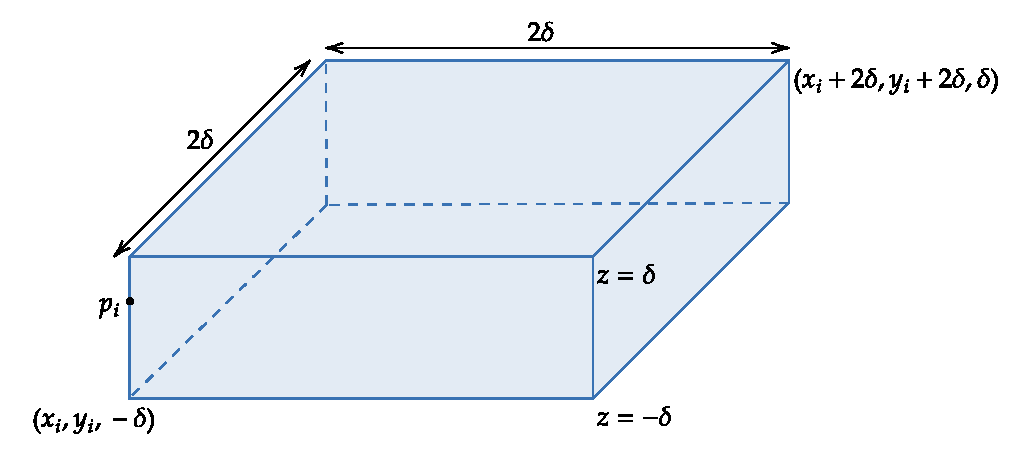
\includegraphics[width=12cm]{images/closest-pari-r3}
	\end{figure}
	
	
	Now by part (a) we know there are at most 64 points in this cube. So we can check for the next $64$. Hence we just check the next 64 points in the sorted $S_1\cup S_2$ and see if there are any points with distance less than $\dl$. Hence the algorithm is:
	
	\begin{algorithm}
		\SetKwComment{Comment}{// }{}
		\DontPrintSemicolon
		\KwIn{Pair of sets $S_1,S_2$ each with $n$ points with in each set any two points have distance at least $\dl$ and further $z-$coordinate of points in $S_1$ in $[0,\dl]$ and of points in $S_2$ in $[-\dl,0]$.}
		\KwOut{Closest pair of ponts, $(P_i,P_j,\delta_0)$ where $\delta_0=d(P_i,P_j)$ with $P_i,P_j\in S_1\cup S_2$}
		\Begin{
		$T_x\longleftarrow S_1\cup S_2$ sorted by $x-$coordinate\;
		$T_y\longleftarrow S_1\cup S_2$ sorted by $y-$coordinate\;
		\For{$i=1,\dots, 2n$}{
	$U_x\longleftarrow $ Next 64 points in $T_x$\;
	$U_y\longleftarrow $ Next 64 points in $T_y$\;
	\For{$\hat{P}\in U_x\cup U_y$}{
\If{$d(P,\hat{P})\leq \dl$}{$\dl\longleftarrow d(P,\hat{P})$\;
$(P_1,P_2)\longleftarrow (P,\hat{P})$}	
}	
	}
\Return{$(P_1,P_2,\dl)$}
	}
\caption{\prb{Find-Closest-2-Sets$(S_1,S_2,\dl)$}}
	\end{algorithm}
In the algorithm instead od checking for a point with distance less than $\dl$ we are checking pair of points with distance less than or equal to $\dl$ this is because we don't have any pair of points in $S_1$ or $S_2$ which are at least $\dl$ distance. So if there is no pair of points in $S_1\cup S_2$ with distance less than $\dl$ we still get a pair of points with distance equal to $\dl$ and that pair points have the shortest distance.\parinf

\textbf{Time Complexity:} Here to sort the points in $S_1\cup S_2$ it takes $O(n\log n)$ time since there are total $2n$ points in $S_1\cup S_2$. Now the for loop runs for $2n$ iterations and in each iterations it is checking for constant number of points and for each point it is doing constant time operations. So each iteration of the loop takes $O(1)$ time and the for loop takes in total $2nO(1)=O(n)$ time. Hence the whole algorithm takes $O(n\log n)$ time.
\item Like in the case of $\bbR^2$ algorithm we will first divide the set of all points into two roughly equal parts which we can do by sorting the points with respect to their $z-$coordinates. Let $\ovz$ be the $\lt\lfloor \frac{n}2\rt\rfloor^{th}$ highest $z-$coordinate. We we partition $S$ into points with $z-$coordinate $< \ovz$ and $\geq z$. Call these sets $S_U$ and $S_D$ respectively. Then run the algorithm recursively on each of those sets. And thus we get a closest pair of points and their distance in each of the smaller sets. So we take the pair of points with the distance equal to  the minimum of those two distances. Call this distance $\dl$. So we only need to check the points from $S$ with $z-$coordinate $\in [\ovz-\dl,\ovz+\dl]$. Call this set of points as $T=S_U^T\sqcup S_D^T$. So $$S_U^T=\{P_i\in S_U\colon z_i\in [\ovz,\ovz+\dl] \}\qquad S_D^T=\{P_i\in S_D\colon z_i\in [\ovz-\dl,\ovz]\}$$
\parinn

Now the situation is almost like the situation in part (b). So we have two sets of points $S_U^T,S_D^T$ each set has at most  $\frac{n}{2}$ points and any two points in any one of the sets has distance at least $\dl$. Then we need to find the closest pair of points in the union of those two sets.

The only change from the situation in part (b) is the now the points in $S_U^T$ have $z-$coordinate   in $[\ovz,\ovz+\dl]$ instead of $[0,\dl]$ and similarly the points in $S_D^T$ have $z-$coordinate in $[\ovz-\dl,\ovz]$ instead of $[-\dl,0]$. Also like in the case of part (b) we don't have to worry about not having a pair of points with their distance $=\dl$. So we have to only look for points with distance less than $\dl$. Therefore we need to do slight change in the algorithm above and then we are good to go.

\begin{algorithm}
	\DontPrintSemicolon
	\KwIn{Set of $n$ points, $S=\{P_i(x_i,y_i,z_i)\mid x_i,y_i,z_i\in\bbR, \ \forall\ i\in[n]\}$.}
	\KwOut{Closest pair of ponts, $(P_i,P_j,\delta)$ where $\delta=d(P_i,P_j)$}
	\Begin{
		\If{$|S|\leq 10$}{Solve by Brute Force (Consider every pair of points)}	
		
		$S^z\longleftarrow S$ sorted by $z-$coordinate\;
		$\ovz\longleftarrow \lfloor \frac{n}{2}\rfloor $ highest $z-$coordinate\;
		$S_U\longleftarrow \{P_i\mid z_i>\bar{z},\ \forall\ i\in[n]\}$\;
		$S_D\longleftarrow \{P_i\mid z_i\leq\bar{z},\ \forall\ i\in[n]\}$\;
		$(P_1^L,P_2^L,\delta^L)\longleftarrow$ \textsc{Find-Closest}($S_U$)\;
		$(P_1^R,P_2^R,\delta^R)\longleftarrow$ \textsc{Find-Closest}($S_D$)\;
		$\delta_{min}\longleftarrow \min\{\delta^L,\delta^R\}$\;
		\If{$\delta_{min}<\delta^L$}{$P_1\longleftarrow P_1^R$, $P_2\longleftarrow P_2^R$}
		
		\Else{$P_1\longleftarrow P_1^L$, $P_2\longleftarrow P_2^L$}
		$S_U^T\longleftarrow \{P_i\mid z_i-\ovz\leq \delta_{min}\}$\;
		$S_D^T\longleftarrow \{P_i\mid \ovz-z_i\leq \delta_{min}\}$\;
		$(P'_1,P'_2,\dl)\longleftarrow \prb{Find-Closest-2-Sets-Mod}\lt(S_U^T,S_D^T,\ovz,\dl_{min}\rt)$\;
		\If{$\dl<\dl_{min}$}{
		\Return{$(P'_1,P'_2,\delta)$}}
	\Else{\Return{$(P_1,P_2,\dl_{min})$}}
	}
	
	\caption{\textsc{Find-Closest}($S$)}
	\label{find-closest-nlog2n}	
\end{algorithm}
Where we describe he \prb{Find-Closest-2-Sets-Mod} algorithm:

	\begin{algorithm}
	\SetKwComment{Comment}{// }{}
	\DontPrintSemicolon
	\KwIn{Pair of sets $S_1,S_2$ each with $n$ points with in each set any two points have distance at least $\dl$ and further $z-$coordinate of points in $S_1$ in $[z,z+\dl]$ and of points in $S_2$ in $[z-\dl,z]$.}
	\KwOut{Closest pair of ponts, $(P_i,P_j,\delta_0)$ where $\delta_0=d(P_i,P_j)$ with $P_i,P_j\in S_1\cup S_2$}
	\Begin{
		$T_x\longleftarrow S_1\cup S_2$ sorted by $x-$coordinate\;
		$T_y\longleftarrow S_1\cup S_2$ sorted by $y-$coordinate\;
		\For{$i=1,\dots, 2n$}{
			$U_x\longleftarrow $ Next 64 points in $T_x$\;
			$U_y\longleftarrow $ Next 64 points in $T_y$\;
			\For{$\hat{P}\in U_xx\cup U_y$}{
				\If{$d(P,\hat{P})<\dl$}{$\dl\longleftarrow d(P,\hat{P})$\;
					$(P_1,P_2)\longleftarrow (P,\hat{P})$}	
			}	
		}
		\Return{$(P_1,P_2,\dl)$}
	}
	\caption{\prb{Find-Closest-2-Sets-Mod$\lt(S_1,S_2,z,\dl\rt)$}}
\end{algorithm}
\parinf

\textbf{Time Complexity:} Let the algorithm takes $T(n)$ to find closest pair of points from $n$ points. To sort the set of points with respect to their $z-$coordinate takes $O(n\log n)$ time. Now forming the sets $S_U$ and $S_D$ takes $O(n)$ time. Now $|S_U|,|S_D|\leq \frac{n}{2}$. Hence in lines 8,9 it takes $T\lt(\frac{n}{2}\rt)$ time. Now line 11-14 it takes constant time. Then again forming the sets $S_U^T,S_D^T$ takes linear time. Then to run the algorithm \prb{Find-Closest-2-Sets-Mod} takes $O(n\log n)$ time. Therefore total time taken is $$T(n)=2T\lt(\frac{n}2\rt)+O(n\log n)$$Hence by \hyperref[p:p1]{Problem \ref{p:p1}: P3 \ref{nlog2n}} we have $T(n)=O(n\log^2n)$. Hence our algorithm takes $O(n\log^2n)$ to find closest pair of points in $\bbR^3$.
\end{enumerate}
}\parinf

[I discussed the solution with Shubham]
%%%%%%%%%%%%%%%%%%%%%%%%%%%%%%%%%%%%%%%%%%%%%%%%%%%%%%%%%%%%%%%%%%%%%%%%%%%%%%%%%%%%%%%%%%%%%%%%%%%%%%%%%%%%%%%%%%%%%%%%%%%%%%%%%%%%%%%%
% Problem 7
%%%%%%%%%%%%%%%%%%%%%%%%%%%%%%%%%%%%%%%%%%%%%%%%%%%%%%%%%%%%%%%%%%%%%%%%%%%%%%%%%%%%%%%%%%%%%%%%%%%%%%%%%%%%%%%%%%%%%%%%%%%%%%%%%%%%%%%%

\begin{problem}{%problem statement
		P9\hfill  (10 marks)
	}{p7% problem reference text
	}
This problem relates to one of the questions asked in class. For any $p, q \geq 1$, and any points $x, y$, and $z \in \mathbb{R}^2$, prove or disprove the following:
		$$
		\|x-y\|_p \leq\|x-z\|_p \Leftrightarrow\|x-y\|_q \leq\|x-z\|_q
		$$

	
	That is, prove or disprove that $y$ is closer to $x$ than $z$ in the $L_p$ distance metric if and only if it is closer to $x$ in the $L_q$ distance metric
	As usual, $\|x-y\|_p=\left(\left(x_1-y_1\right)^p+\left(x_2-y_2\right)^p\right)^{1 / p}$.
\end{problem}
\solve{
	This question reduces to showing for any two points $x,y\in\bbR^2$ if the following is true of not $$\|x\|_p\leq \|y\|_p\iff \|x\|_q\leq \|y\|_q$$This is not true. Take $p=1$, $q=2$. And $x=(1,0)$ and $y=(0.55,0.55)$. Then $\|x\|_1=\|x\|_2=1$. But $\|y\|=1.1$, $\|y\|=0.55\sqrt{2}<1$. Hence $\|x\|_1<\|y\|_1$ but $\|x\|_2>\|y\|_2$. Hence the above claim is not true.
}
\end{document}
